%\documentclass{standalone}
%\usepackage[dvipsnames]{xcolor}
%\usepackage{tikz}
%\usepackage{amsmath}
%\usepackage{siunitx}
%\usepackage{pgfplots}

%\usetikzlibrary{calc}
%\usetikzlibrary{decorations.pathmorphing}

%\definecolor{light-gray}{gray}{0.9}

%\definecolor{red}{HTML}{d62728}
%\definecolor{orange}{HTML}{ff7f0e}
%\definecolor{green}{HTML}{2ca02c}
%\definecolor{blue}{HTML}{1f77b4}
%\definecolor{purple}{HTML}{9467bd}
%\definecolor{light-gray}{gray}{0.9}

%\begin{document}
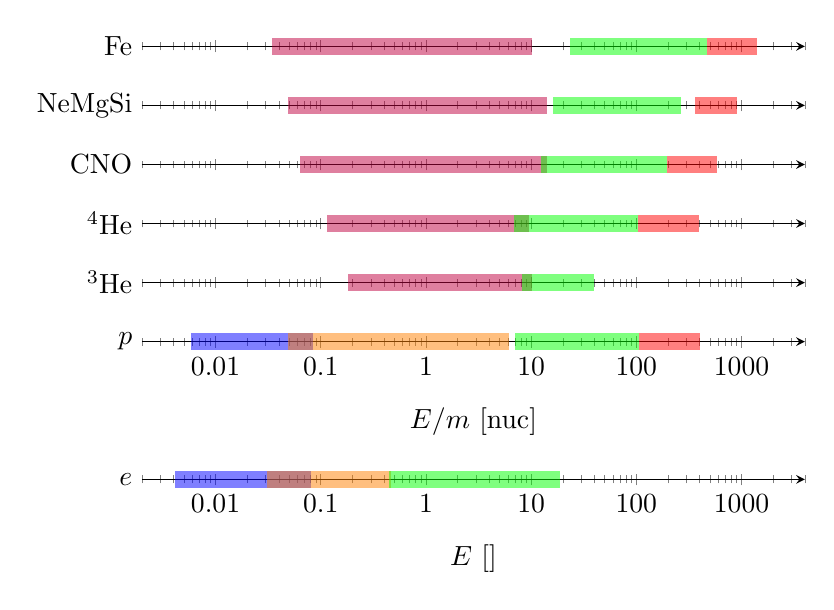
\begin{tikzpicture}
	\def\xmin{0.002}
	\def\xmax{4000}

	% EPT energy ranges, based on calibration as of 2020-10-01
	% ELECTRONS
	\begin{semilogxaxis}[xmin=\xmin, xmax=\xmax, axis x line=middle, hide y axis, ymin=-2,ymax=2,
					 height=2cm, width=10cm,
					 xlabel={$E$ [\si{\mega\electronvolt}]},
					 x label style={at={(axis description cs:0.5,-1.2)},anchor=north},clip=false,
					 log ticks with fixed point, x tick label style={/pgf/number format/1000 sep={}},yshift=0.25cm]
		\fill[blue, opacity=0.5] (axis cs:0.0041, -1) rectangle (axis cs:0.080, 1);
		\fill[orange, opacity=0.5] (axis cs:0.031, -1) rectangle (axis cs:0.47, 1);
		\fill[green, opacity=0.5] (axis cs:0.45, -1) rectangle (axis cs:18.8, 1);
		\node[left] at (axis cs:\xmin, 0) {$e$};
	\end{semilogxaxis}
	
	% PROTONS
	\begin{semilogxaxis}[xmin=\xmin, xmax=\xmax, axis x line=middle, hide y axis, ymin=-2,ymax=2,
	height=2cm, width=10cm, 
	xlabel={$E/m$ [\si{\mega\electronvolt\per nuc}]},
	x label style={at={(axis description cs:0.5,-1.2)},anchor=north},
	yshift=2cm, clip=false,
	log ticks with fixed point, x tick label style={/pgf/number format/1000 sep={}}]
		\fill[blue, opacity=0.5] (axis cs:0.0058, -1) rectangle (axis cs:0.085, 1);
		\fill[orange, opacity=0.5] (axis cs:0.049, -1) rectangle (axis cs:6.1, 1);
		\fill[green, opacity=0.5] (axis cs:7.0, -1) rectangle (axis cs:105, 1);
		\fill[red, opacity=0.5] (axis cs:105, -1) rectangle (axis cs:401.13, 1);
		%\fill[purple, opacity=0.5] (axis cs:0.24, 1) rectangle (axis cs:9.4, 3);
		\node[left] at (axis cs:\xmin, 0) {$p$};
	\end{semilogxaxis}
	
	% 3He
	\begin{semilogxaxis}[xmin=\xmin, xmax=\xmax, axis x line=middle, hide y axis, ymin=-2,ymax=2,
	height=2cm, width=10cm, xticklabels={,,},
	yshift=2.75cm, clip=false]
		\fill[purple, opacity=0.5] (axis cs:0.18, -1) rectangle (axis cs:10.2, 1);
		\fill[green, opacity=0.5] (axis cs:8.1, -1) rectangle (axis cs:39.7, 1);
		\node[left] at (axis cs:\xmin, 0) {$^3$He};
	\end{semilogxaxis}
	
	% 4He
	\begin{semilogxaxis}[xmin=\xmin, xmax=\xmax, axis x line=middle, hide y axis, ymin=-2,ymax=2,
	height=2cm, width=10cm, xticklabels={,,},
	yshift=3.5cm, clip=false]
		%\fill[orange, opacity=0.5] (axis cs:6.37, 1) rectangle (axis cs:24.51, 3);
		\fill[purple, opacity=0.5] (axis cs:0.115, -1) rectangle (axis cs:9.493, 1);
		\fill[green, opacity=0.5] (axis cs:6.877, -1) rectangle (axis cs:104, 1);
		\fill[red, opacity=0.5] (axis cs:104, -1) rectangle (axis cs:392.84, 1);
		\node[left] at (axis cs:\xmin, 0) {$^4$He};
	\end{semilogxaxis}
	
	% CNO
	\begin{semilogxaxis}[xmin=\xmin, xmax=\xmax, axis x line=middle, hide y axis, ymin=-2,ymax=2,
	height=2cm, width=10cm, xticklabels={,,},
	yshift=4.25cm, clip=false]
		\fill[purple, opacity=0.5] (axis cs:0.064, -1) rectangle (axis cs:14.13, 1);
		\fill[green, opacity=0.5] (axis cs:12.54, -1) rectangle (axis cs:197, 1);
		\fill[red, opacity=0.5] (axis cs:197, -1) rectangle (axis cs:578.37, 1);
		\node[left] at (axis cs:\xmin, 0) {CNO};
	\end{semilogxaxis}
	
	% NeMgSi
	\begin{semilogxaxis}[xmin=\xmin, xmax=\xmax, axis x line=middle, hide y axis, ymin=-2,ymax=2,
	height=2cm, width=10cm, xticklabels={,,},
	yshift=5cm, clip=false]
		\fill[purple, opacity=0.5] (axis cs:0.049, -1) rectangle (axis cs:14.13, 1);
		\fill[green, opacity=0.5] (axis cs:16.2, -1) rectangle (axis cs:268.42, 1);
		\fill[red, opacity=0.5] (axis cs:358, -1) rectangle (axis cs:915.03, 1);
		\node[left] at (axis cs:\xmin, 0) {NeMgSi};
	\end{semilogxaxis}
	
	% Fe
	\begin{semilogxaxis}[xmin=\xmin, xmax=\xmax, axis x line=middle, hide y axis, ymin=-2,ymax=2,
	height=2cm, width=10cm, xticklabels={,,},
	yshift=5.75cm, clip=false]
		\fill[purple, opacity=0.5] (axis cs:0.0346, -1) rectangle (axis cs:10.29, 1);
		\fill[green, opacity=0.5] (axis cs:23.66, -1) rectangle (axis cs:465.7, 1);
		\fill[red, opacity=0.5] (axis cs:465.8, -1) rectangle (axis cs:1388.40, 1);
		\node[left] at (axis cs:\xmin, 0) {Fe};
	\end{semilogxaxis}
\end{tikzpicture}
%\end{document}